\documentclass{article}

\usepackage[a4paper, top=35mm, bottom=40mm, right=30mm, left=30mm]{geometry}
\usepackage[ngerman]{babel}
\usepackage[utf8x]{inputenc}
\usepackage[T1]{fontenc}
\usepackage{mathtools}
\usepackage{textcomp}
\usepackage{graphicx}
\usepackage{tabularx}
\usepackage{amssymb}
\usepackage{pifont}
\newcommand{\cmark}{\ding{51}}%
\newcommand{\xmark}{\ding{55}}%
\setlength{\parindent}{0pt}
\linespread{1.6}

\title{Crawling von Datenschutzerklärung-Historien}
\author{Alexander Prull, Jörn-Henning Daug, Simon Kaleschke}
\date{05. Februar 2017}

\begin{document}
	
	\maketitle
	
	\section{Projektbeschreibung}
	Das Praktikumsthema "Crawling von Datenschutzerklärung-Historien"{} beschäftigt sich mit den Datenschutzerklärungen ausgewählter Websites. Die Websites sollen regelmäßig auf neue Versionen geprüft werden. Neue Versionen sammelt der Crawler in einer Datenbank. Die verschiedenen Datenschutzerklärungen eines Unternehmens werden dann auf einer Website gegenübergestellt und Veränderungen sichtbar gemacht.
	\section{Lösungsansatz}
	Die Software ist in drei Teile aufgeteilt: Frontend, Backend und Extraktion. Das Frontend übernimmt dabei die grafische Oberfläche des Projekts. Die ausgewählten Versionen der Datenschutzerklärungen sind hier gegenübergestellt. Ein Diff-Tool macht die Veränderungen erkennbar.
	Die Extraktion sammelt durch einen Crawler die Datenschutzerklärungen der Unternehmen ein und legt sie in die ausgewiesene Datenbank.
	Das Backend übernimmt die Kommunikation zwischen Datenbank und Frontend und startet in regelmäßigen Abständen die Extraktion.
	\section{Softwarearchitektur}
	Die einzelnen Komponenten sind jeweils in einem Ordner abgelegt. Im Ordner \textit{script} liegen die Dateien für das Crawling und die Datenbank, \textit{tmc\_frontend} enthält das Frontend und \textit{tmc\_backend} dementsprechend das Backend.	
	Im folgenden werden die einzelnen Komponenten des Projekts genauer beschrieben.
	
	\subsection{Frontend}
	Die Weboberfläche zur Darstellung und zum Vergleich der Datenschutzerklärungen bildet das Frontend des Projektes. Für die Darstellung wurde ein Onepager erstellt, der aus drei Elementen besteht. Eine ausfahrbare Sidebar auf der linken Seite dient zur Auswahl der gewünschten Website.\newline
Im oberen Bereich der Seite zeigt ein Zeitstrahl anschließend alle verfügbaren Datenschutzerklärungen anhand ihrer Eintragungsdaten an. Darunter befinden sich zwei Textfelder.\newline
Durch Klicken auf den gewünschten Eintrag im Zeitstrahl wird der Text als Referenz in das linke Feld geladen. Wählt man nun ein zweites Datum aus, startet das Diff-Tool und zeigt im rechten Feld die Unterschiede der beiden Datenschutzerklärungen an. Dabei steht rot für „nicht mehr vorhanden“, grün für „neu hinzugekommen“ und grau für „unverändert“.
Das Frontend baut sich aus \textit{bower}-Komponenten auf und wird durch \textit{bootstrap} optisch optimiert. Die Funktionalität im Frontend wird durch \textit{AngularJS} unterstützt. Anfragen über zwei REST-Schnittstellen an das Backend importieren die nötigen Informationen.
	\subsection{Backend}
	Das Backend ist ein Maven-Projekt und besteht aus vier Paketen: \textit{server\_core},  \textit{resources}, \textit{representation} und \textit{tools}.\newline 
	Zentraler Startpunkt ist der \textit{server\_core}. In diesem Paket befindet sich die Hauptklasse \textit{Start.java}. Sie startet zwei Threads für den Server und den Crawler. Der Server ist nach dem Start unter der dort hinterlegten Server-IP und dem Port 8080 erreichbar und wartet auf Anfragen des Frontends. Der Crawler startet die Extraktion (\textit{crawl.rb}) regelmäßig. In der Voreinstellung einmal am Tag.\newline 
	Wenn das Frontend eine Anfrage stellt, wird das Paket \textit{tools} aktiv. In diesem befindet sich die Datenbankinitialisierung, sowie die Klassen für die SQL-Anfragen zum Ausliefern eines gewünschten Textes einer Datenschutzerklärung(\textit{TextLoader.java}) und aller Datumswerte der abgespeicherten Versionen (\textit{DateLoader.java}) eines Unternehmens.\newline 
	Das Paket \textit{resources} wandelt die Ergebnisse aus dem \textit{tools}-Paket in JSONs um und ist zuständig für den Aufbau einer REST-Schnittstelle auf einer URL und die Auslieferung der JSONs an diese Website.\newline 
	Die Klassen aus dem letzten Paket \textit{representation} bauen die Objekte auf, die an die URLs übermittelt werden. Das Objekt \textit{Texts} besteht aus dem Text der Datenschutzerklärung und dem Datum der Veröffentlichung. Das Objekt \textit{Date} enthält eine ID, einen Datumswert für eine bessere Verarbeitung im Code (\textit{SYSTEM\_DATE}) und einen Datumswert für eine bessere Lesbarkeit (\textit{DISPLAY\_DATE}).\newline
	Das Klassendiagramm zum Backend ist als Abbildung 2 im Anhang hinterlegt.
	 
	
	\subsection{Extraktion}
	Die Ruby-Struktur zur Extraktion der Datenschutzhistorien funktioniert folgendermaßen:
	
	Vom Backend aus wird \textit{crawl.rb} aufgerufen. Dieses Skript beinhaltet alle Einstellungen zur Extraktion von jeder Webseite. Es sendet diese Einstellungen an \textit{PrivacyExtractor.rb}, das die Extraktion dann vollzieht. Hierfür bezieht es Links zu älteren Versionen entweder vom Archiv der Webseite selbst, oder mit \textit{ArchiveExtractor.rb} von dem Internetarchiv \textit{archive.org}. Der Inhalt jeder Seite wird extrahiert, auf die notwendigen Elemente zugeschnitten und formatiert. Zuletzt werden mit \textit{PrivacyDiffer.rb} die extrahierten Texte auf Unterschiede untersucht und gegebenenfalls in einer Datenbank abgespeichert. Die Datumswerte und Texte aus der fertigen Datenbank können vom Frontend abgefragt werden.
	
	Weitere Informationen sind auf der Abbildung \ref{fig:uml-ex} auf Seite \pageref{fig:uml-ex} zu finden.
	
	\section{Bedienungsanleitung}
	Die folgende Bedienungsanleitung enthält einen kurzen Einblick über die verwendeten Software-Komponenten, die Einrichtung und Start des Servers, sowie eine Erklärung des Crawling-Prozess.
	\subsection{Vorbereitung}
	Damit die Software reibungslos läuft, werden folgende vorinstallierte Pakete erwartet:
	
	Für das Frontend:
	\begin{itemize}
		\item NodeJS(Npm/Bower)
		\item Bootstrap
		\item vis
		\item diff (Npm) bzw. jsdiff (Bower)
		\item jQuery
	\end{itemize}

	Für das Backend:
	\begin{itemize}
		\item Java
		\item SQLite3
		\item Maven
	\end{itemize}

	Für die Extraktion:
	\begin{itemize}
		\item Ruby 2.3.1 oder höher.
		\item Die Ruby-Gems \textit{date, open-uri, open\_uri\_redirections, nokogiri, rubygems, sqlite3, json, differ}.
	\end{itemize}

	Tragen sie außerdem in der Datei \textit{config.ppp} den von Ihnen gewünschten Pfad für die Ergebnisdatenbank ein. (Standard ist \textit{$\sim$/html/script/policies.db}) 
	\subsection{Server einrichten}
	Damit das Backend die JSONs für das Frontend bereitstellen kann, muss in der Klasse \textit{ServerStarter.java} im Paket \textit{server\_core} die Server-IP eingetragen werden. Um die Uhrzeit zu ändern, an dem der Crawling-Prozess gestartet wird, müssen im selben Paket in der Klasse \textit{CrawlerStarter.java} die entsprechenden Variablen abgeändert werden.\newline
	Zum Erstellen einer \textit{jar} muss im Ordner \textit{tmc\_backend} der Befehl \textit{mvn clean package} erfolgen. Eine fertige \textit{jar} liegt bereits im Unterordner \textit{target}. 
	\subsection{Serverstart und allgemeiner Programmablauf}
	Gestartet wird der Backend-Server mit der \textit{Start.java}-Klasse durch die \textit{jar} im  Ordner \textit{target}. Diese Klasse ist als Hauptklasse in der \textit{pom.xml} des Maven-Projekts hinterlegt. Danach starten sich zwei Threads für den Server und den Crawler. Der Server steht danach für Anfragen aus dem Frontend bereit. Ohne den Start der \textit{jar} kann das Frontend nicht auf die Datenbank zugreifen. \newline Der Crawling-Prozess wird einmal täglich durchgeführt. Zum Beenden bzw. Deaktivieren des Crawlers muss \textit{Enter} gedrückt werden. Durch wiederholtes Drücken der \textit{Enter}-Taste wird auch der Server beendet.
	\subsection{Webseite einzeln crawlen}
	Normalweise wird der Aufruf zur Extraktion vom Backend aus gestartet. Wollen Sie jedoch eine einzelne Webseite crawlen, gehen sie folgendermaßen vor:
	\begin{enumerate}
		\item Versichern Sie sich, dass die Webseite und zugehörige Optionen im Quellcode vermerkt sind (siehe dazu Abschnitt \ref{sec:add-site}).
		\item Sind noch keine Informationen zu der Webseite vorhanden oder wollen Sie alle Informationen von null an neu generieren lassen, wechseln sie in den Ordner \textit{script} und starten sie den Aufruf \textit{ruby crawl.rb webseite fetch}. Wollen sie bspw. alle Informationen für Google neu generieren lassen, ersetzen sie im Aufruf \textit{webseite} durch \textit{google}.
		\item Wollen Sie nun überprüfen, ob eine neue Version verfügbar ist, starten Sie den Aufruf \textit{ruby crawl.rb webseite update}.
	\end{enumerate}
	
	\subsection{Datenbankstruktur}
		Die SQLite-Datenbank hat folgende Spalten:
		
		\begin{tabularx}{\textwidth}{|r|X|}
			\hline
			\textbf{Spalte} & \textbf{Bedeutung} \\ \hline \hline
			ID & Primärschlüssel. \\ \hline
			SYSTEM\_DATE & Datum, an dem die Datenschutzhistorie in dem aktuellen Zustand war.\\ \hline
			DISPLAY\_DATE & Gleiches Datum in benutzerfreundlicher Schreibweise. \\ \hline
			LINK & Hyperlink, wo die extrahierte Historie zu finden ist.\\ \hline
			CONTENT & Der extrahierte Plaintext.\\ \hline
		\end{tabularx}
	
	
	\section{Ergebnisse} 
	
	Das Projekt ist in der Lage eigenständig und dauerhaft 20 Websites zu crawlen und dadurch die Datenbank aktuell zu halten. Eine Liste aller gecrawlten Webseiten ist auf Abbildung \ref{fig:crawl-tab} auf Seite \pageref{fig:crawl-tab} zu finden.
	\newline
	Die Weboberfläche besitzt eine Sidebar, einen Zeitstrahl und zwei Textfelder. Die Datenschutzerklärungen der 20 gecrawlten Websites sind über die jeweiligen Reiter der Sidebar aufrufbar. Auf dem Zeitstrahl entsteht dann eine Übersicht, wann die Website ihre Datenschutzerklärung aktualisiert hat. Wählt man ein Datum aus, erscheint die Datenschutzerklärung als Text und kann mit einem anderen Zeitpunkt über das Diff-Tool verglichen werden.
	
	\section{Einschränkungen}
	Das Projekt ist auf 20 Websites angesetzt worden. Da die Strukturen der Websites immer unterschiedlich sind, muss auch der Crawler darauf abgestimmt sein. Weitere Websites müssen also jedes Mal neu untersucht und die Crawling-Routine programmiert werden.\newline
	Sollte sich in Zukunft die Struktur einer der 20 Websites ändern, so funktioniert der Crawling-Prozess nicht mehr. Eine Wartung des Crawlers muss einkalkuliert werden.
	\section{Erweiterungsmöglichkeiten}
	\subsection{Daten weiterverarbeiten}
	Die gewonnenen Daten in der Datenbank können unabhängig von der Webseite vielseitig weiterverwendet werden. So wäre bspw. die Anbindung an weitere Anwendungsprogramme denkbar, z.B. zur Bewertung der Datenqualität oder zur Suche nach Schlüsselwörtern.
	\subsection{Webseite hinzufügen}
	\label{sec:add-site}
	Wenn Sie eine Webseite zum Tool hinzufügen möchten, so brauchen Sie i.A. den Namen der Webseite und einen Hyperlink zur Webseite, auf der die Datenschutzerklärung zu finden ist. Wie weiter vorzugehen ist, wird im folgenden beschrieben:
	\subsubsection{Frontend}
	Alle Strukturen zum Aufbau des Frontends sind durch AngularJS weitestgehend dynamisch und auf Bedarf anpassbar. Die Reiter in der Sidebar passen sich der Daten aus der Restschnittstelle an und alle weiteren Websiten sollten ohne Probleme integriert werden.
	\subsubsection{Extraktion}
	Eine neue Website ändert nichts an der Struktur des Backends. Es muss aber die Extraktion bearbeitet werden. Fügen Sie in \textit{crawl.rb} den Namen der Webseite, den Link, den Namen der Tabelle, in der die Informationen gespeichert werden sollen, wie die HTML-Struktur zu modifizieren ist, etc. ein. Näheres wird mit Beispielen im Skript selbst erläutert.
	\subsection{Weitere Daten aus Datenbank abfragen}
	Wenn dem Frontend weitere JSONs zur Verfügung gestellt werden sollen, gehen Sie wie folgt vor: Erstellen Sie eine neue Klasse für ein Objekt im Paket \textit{representation}. Danach formulieren Sie eine SQL-Anfrage in einer Klasse des Paketes \textit{tools}. Außerdem müssen dort die Ergebnisse das Objekt aus \textit{representation} befüllen und in einer \textit{List<t>} gesammelt werden. Zum Schluss erstellen Sie im Paket \textit{resources} eine neue Ressource, an die die \textit{List<t>} als JSON ausgeliefert wird.
	\newpage
	\section{Anhang}
	\begin{figure}[ht]
		\centering
		
		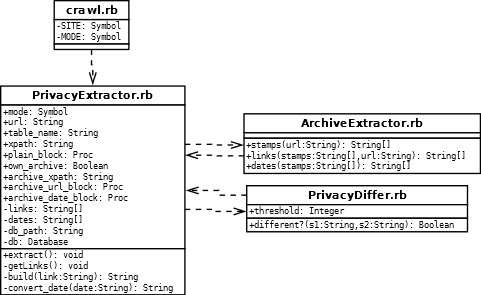
\includegraphics[width=0.75\textwidth]{extraction}
		\caption{Architektur Extraktion}
		\label{fig:uml-ex}
	\end{figure}
	\newpage
	\begin{figure}[ht]
		\centering
		
		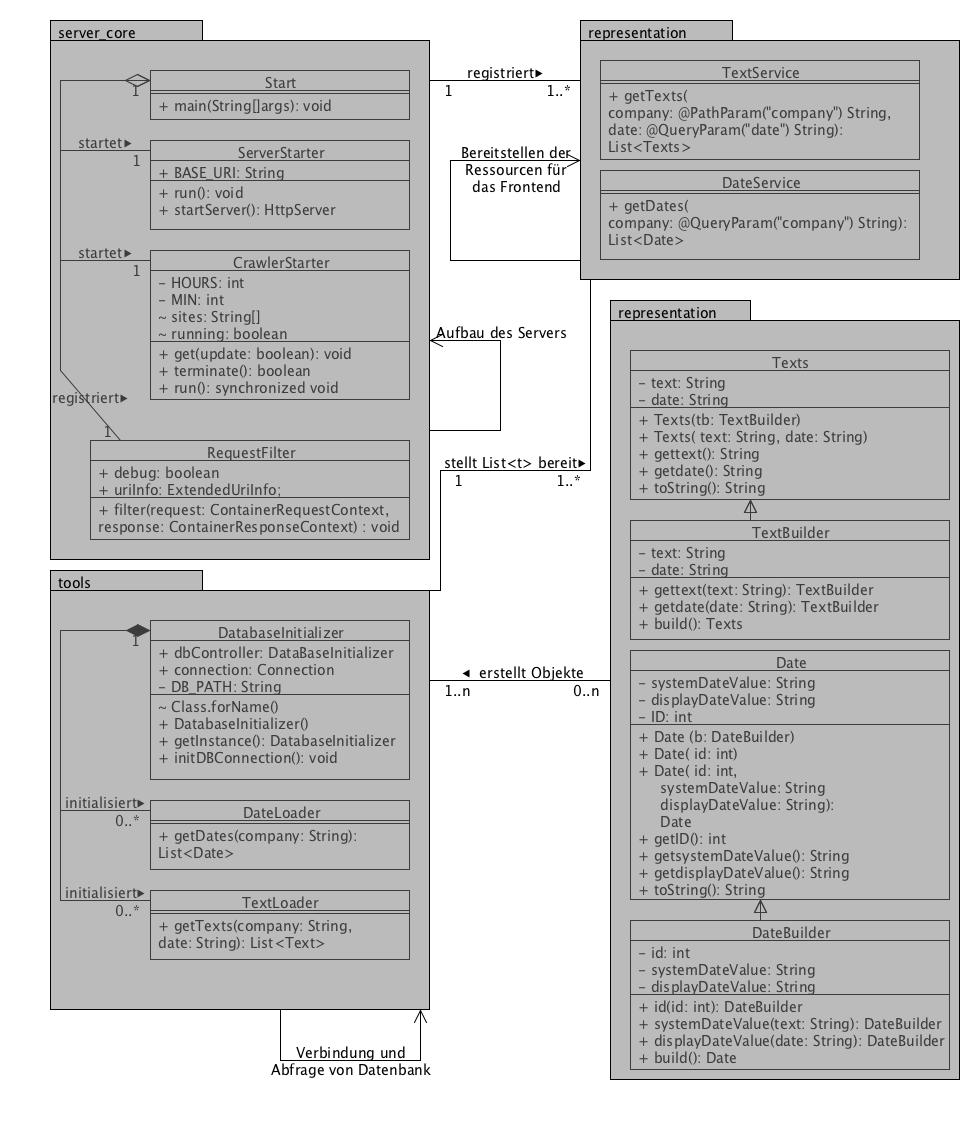
\includegraphics[width=1\textwidth]{tmc_backend}
		\caption{Architektur Backend}
		\label{fig:uml-ex}
	\end{figure}
	\begin{figure}[ht]
		\centering
		\begin{tabularx}{\textwidth}{|r|c|c|c|X|}
			\hline
			\textbf{Firma} & \textbf{Eigenes Archiv} & \textbf{Versionen} & \textbf{Zeitspanne} & \textbf{Qualität} \\ \hline \hline
			Alternate & \xmark & 7 & 08/2014 - 07/2016 &  0.9 \\ \hline
			Amorelie & \xmark & 11 & 01/2013 - 10/2016 &  0.7 \\ \hline
			Apple & \xmark & 12 & 09/2014 - 09/2016 &  1.0 \\ \hline
			Burgerking & \xmark & 2 & 02/2015 - 12/2016 &  0.7 \\ \hline
			Edeka & \xmark & 4 & 11/2014 - 10/2016 &  0.7 \\ \hline
			Google & \cmark & 22 & 06/1999 - 01/2017 &  0.8 \\ \hline
			Microsoft & \xmark & 7 & 02/2016 - 01/2017 &  0.9 \\ \hline
			Payback & \xmark & 10 & 09/2011 - 10/2016 &  0.9 \\ \hline
			Paypal & \xmark & 2 & 04/2014 - 11/2016 &  0.9 \\ \hline
			RocketbeansTV & \xmark & 4 & 10/2014 - 09/2016 &  1.0 \\ \hline
			Steam & \xmark & 3 & 09/2012 - 11/2016 &  0.8 \\ \hline
			Subway & \xmark & 3 & 05/2016 - 10/2016 &  0.9 \\ \hline
			Süddeutsche & \xmark & 1 & 04/2015 - 04/2015 &  0.2 \\ \hline
			Trivago & \xmark & 1 & 04/2016 - 04/2016 &  0.7 \\ \hline
			Twitter & \cmark & 10 & 05/2007 - 01/2016 &  0.8 \\ \hline
			Uni Leipzig & \xmark & 1 & 06/2013 - 06/2013 &  0.5 \\ \hline
			Vine & \xmark & 5 & 03/2013 - 01/2017 &  1.0 \\ \hline
			WhatsApp & \cmark & 2 & 07/2012 - 01/2017 &  0.9 \\ \hline
			Wikimedia & \cmark & 4 & 06/2006 - 06/2014 &  1.0 \\ \hline
			Zalando & \xmark & 3 & 09/2010 - 11/2012 &  0.9 \\ \hline
		\end{tabularx}
		\caption{Übersicht gecrawlte Webseiten}
		\label{fig:crawl-tab}
	\end{figure}
	
\end{document}